%
% $RCSfile$
%
% Copyright (c) 2005-2006. Christian Heller. All rights reserved.
%
% Permission is granted to copy, distribute and/or modify this document
% under the terms of the GNU Free Documentation License, Version 1.1 or
% any later version published by the Free Software Foundation; with no
% Invariant Sections, with no Front-Cover Texts and with no Back-Cover
% Texts. A copy of the license is included in the section entitled
% "GNU Free Documentation License".
%
% http://www.cybop.net
% - Cybernetics Oriented Programming -
%
% http://www.resmedicinae.org
% - Information in Medicine -
%
% Version: $Revision$ $Date$ $Author$
% Authors: Christian Heller <christian.heller@tuxtax.de>
%

\section{Introduction}
\label{introduction_heading}

\emph{Software Development} as one field of the science of \emph{Informatics}
has delivered many innovative concepts in its meanwhile rather long history.
While some of them (like procedural-, but also object-oriented programming) are
already in use for decades, others (like concerns, components or ontologies)
are still quite young and yet have to prove their suitability for certain tasks
of software development, or yet have to get accepted by the business world.

This article reports about the results of a five-year-long research work within
the area of software development, in particular software design.

%
% $RCSfile$
%
% Copyright (c) 2002-2006. Christian Heller. All rights reserved.
%
% Permission is granted to copy, distribute and/or modify this document
% under the terms of the GNU Free Documentation License, Version 1.1 or
% any later version published by the Free Software Foundation; with no
% Invariant Sections, with no Front-Cover Texts and with no Back-Cover
% Texts. A copy of the license is included in the section entitled
% "GNU Free Documentation License".
%
% http://www.cybop.net
% - Cybernetics Oriented Programming -
%
% http://www.resmedicinae.org
% - Information in Medicine -
%
% Version: $Revision$ $Date$ $Author$
% Authors: Christian Heller <christian.heller@tuxtax.de>
%

\subsection{Software Crisis}
\label{software_crisis_heading}

An early question in software engineering was how to write programs that control
a computer system's \emph{Hardware} correctly and efficiently. Over time, the
importance of hardware shifted in favour of \emph{Software} which nowadays
contains most of the logic needed to run an application on a computer system.
Consequently, much more research emphasis is now placed on the finding of clever
modelling concepts that help writing correct and effective, stable and robust,
flexible and maintainable, secure software. Another objective is to increase the
effectiveness and lessen the expenditure of cost and time in software development
projects, by \emph{reusing} (pieces of) software.

The past 40 years have delivered numerous helpful concepts, for instance
\emph{Structure} and \emph{Procedure}, \emph{Class} and \emph{Inheritance},
\emph{Pattern} and \emph{Framework}, \emph{Component} and \emph{Concern}, and
many more. They undoubtedly have moved software design far forward. Nevertheless,
the dream of true componentisation and full reusability has not been reached.
Czarnecki \cite{czarnecki} identifies problems in the four areas: \emph{Reuse},
\emph{Adaptability} (\emph{Flexibility}), management of \emph{Complexity} and
\emph{Performance}.

Modern software is very \emph{complex}. It runs on different hardware platforms,
uses multiple communication paradigms and offers various user interfaces. Many
tools and methods assist experts as well as engineers in creating and maintaining
software but do they not seem sufficient to cope with the complexity so that
often, systems still base on buggy source code causing:

\begin{itemize}
    \item[-] False Results
    \item[-] Memory Leaks
    \item[-] Endless Loops
    \item[-] Weak Performance
    \item[-] Security Holes
\end{itemize}

Are these exclusively the fault of software developers? Or, are the used
concepts perhaps insufficient? Using the same, allegedly unsatisfying concepts
caused some people to talk about an ongoing \emph{Software Crisis}, sometimes
\emph{Complexity Crisis}, affecting not only high-level application programming,
but also low-level microchip design \cite{daene}.

However, answers are not easy to find. Software design is \emph{Arts} and
\emph{Engineering}, at the same time. Not everything is or can be regulated by
rules. It is true, developers have to stick to a set of design rules -- and
tools that support their usage exist -- but they also have to be very creative.
All the time, they have to have new, innovative ideas and apply them to software.
This is what makes the creation, integration, test and maintenance of software
so difficult. There is not really a uniform way of treating it.

%
% $RCSfile: motivation.tex,v $
%
% Copyright (C) 2002-2008. Christian Heller.
%
% Permission is granted to copy, distribute and/or modify this document
% under the terms of the GNU Free Documentation License, Version 1.1 or
% any later version published by the Free Software Foundation; with no
% Invariant Sections, with no Front-Cover Texts and with no Back-Cover
% Texts. A copy of the license is included in the section entitled
% "GNU Free Documentation License".
%
% http://www.cybop.net
% - Cybernetics Oriented Programming -
%
% http://www.resmedicinae.org
% - Information in Medicine -
%
% Version: $Revision: 1.1 $ $Date: 2008-08-19 20:41:07 $ $Author: christian $
% Authors: Christian Heller <christian.heller@tuxtax.de>
%

\section{Motivation}
\label{motivation_heading}
\index{Motivation}
\index{Abstraction Gaps}
\index{Misleading Tiers}
\index{Modelling Mistakes}
\index{Inter-Disciplinary Effort}

To the issues that this work has with some state-of-the-art solutions belong in
particular three things:

\begin{enumerate}
    \item \emph{Abstraction Gaps} in Software Engineering Process (chapter
        \ref{software_engineering_process_heading})
    \item \emph{Misleading Tiers} in Physical Architecture (chapter
        \ref{physical_architecture_heading})
    \item \emph{Modelling Mistakes} in Logical Architecture (chapter
        \ref{logical_architecture_heading})
\end{enumerate}

The traversing of abstraction gaps in a software engineering process belongs to
the main difficulties in software development, and causes considerable cost-
and time effort. It necessitates a steady synchronisation between domain
experts and application system developers, because their responsibilities
cannot be clearly separated and interests often clash. A first objective of
this work is therefore to contribute to closing these gaps, especially the one
existing between a designed system architecture and the implemented source
code.

The misinterpretation of the physical tiers in an information technology
environment often leads to wrong-designed software architectures. Logical
layers are adapted to physical tiers (frontend, business logic and backend) and
differing patterns are used to implement them. Instead, systems should be
designed in a way that allows the usage of a unified translator architecture,
so to give every application system the capability to communicate universally
by default, which is the second objective of this work.

Several well-known issues exist with the modelling of logical system
architectures, for example: fragile base class problem, container inheritance,
bidirectional dependencies, global data access. These and others more result
from using wrong principles of knowledge abstraction, like the bundling of
attributes and methods in one class, as suggested by object oriented
programming, or the equalising of structural- and meta information in a model.
A third and final aim of this work is therefore to closer investigate the basic
principles and concepts after which current software systems are created, and
to search for new ideas and concepts, with the objective of finding a universal
type structure (knowledge schema).

On its search for new ideas, this work intentionally tries to cross the borders
to other scientific disciplines. It can therefore also be called an
\emph{inter-disciplinary} effort. Results from many different sciences are
applied to software engineering. Most emphasis, however, is placed on the
comparison between human- and computer systems. Nature has always been a good
teacher and its principles have often been copied; so does this work.

%
% $RCSfile$
%
% Copyright (c) 2005-2006. Christian Heller. All rights reserved.
%
% Permission is granted to copy, distribute and/or modify this document
% under the terms of the GNU Free Documentation License, Version 1.1 or
% any later version published by the Free Software Foundation; with no
% Invariant Sections, with no Front-Cover Texts and with no Back-Cover
% Texts. A copy of the license is included in the section entitled
% "GNU Free Documentation License".
%
% http://www.cybop.net
% - Cybernetics Oriented Programming -
%
% http://www.resmedicinae.org
% - Information in Medicine -
%
% Version: $Revision$ $Date$ $Author$
% Authors: Christian Heller <christian.heller@tuxtax.de>
%

\subsection{Idea}
\label{idea_heading}

On its search for new concepts, this work intentionally tried to cross the
borders to other scientific disciplines. The idea behind is as simple as it is
helpful: \textit{Inspect solutions of various other disciplines of science,
phenomenons of nature, and apply them to software engineering \ldots\ in order
to find out if weaknesses existing in traditional techniques can be eliminated.}
Since results from many different sciences were applied to software engineering,
the work can be called an \emph{inter-disciplinary} effort. Most emphasis,
however, was placed on the comparison between human- and computer systems, which
is why this work was given the name \emph{Cybernetics Oriented Programming}
(CYBOP). Nature has always been a good teacher and its principles have often
been copied; so did this work.

\begin{figure}[ht]
    \begin{center}
        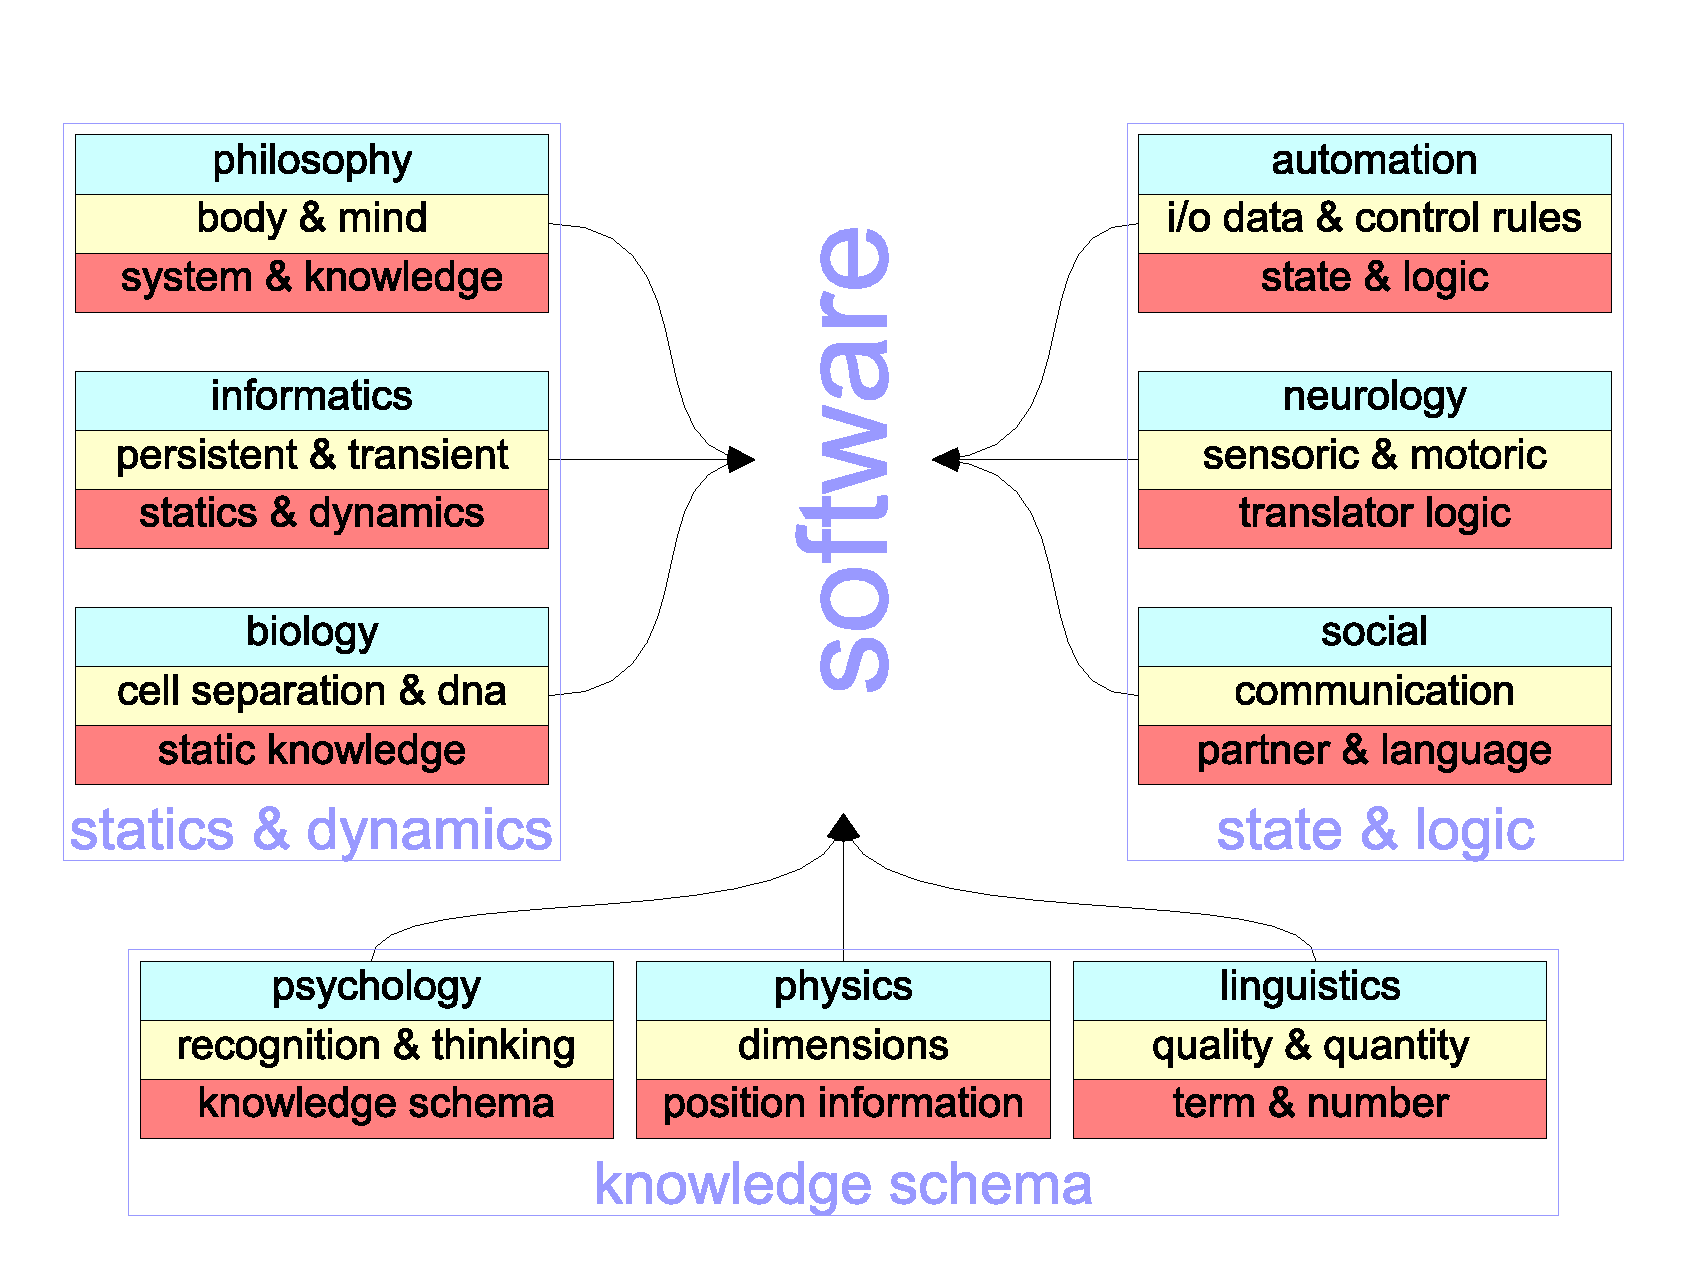
\includegraphics[scale=0.2]{vector/mindmap.eps}
        \caption{Mindmap of Influential Sciences}
        \label{mindmap_figure}
    \end{center}
\end{figure}

Figure \ref{mindmap_figure} shows some of the sciences whose principles were
considered in this work. The name of a field of science is shown on top of each
box. Made observations are mentioned below, in the middle. The resulting design
recommendations for software can be found at the bottom of each box. The
recommendations are grouped into those that justify a separation of
\emph{Statics and Dynamics} (left-hand side), a new kind of
\emph{Knowledge Schema} (lower part of the figure) and a distinction between
\emph{State and Logic} models (right-hand side).

It has to be mentioned though, that only some of the principles underlying a
specific field of science were considered in the figure and in more detail later
in this article. The figure does by no means claim to be complete. The shown
observations are only those that seemed promising in the context of software
design. The existence of persistent and transient data, for example, is only
one of many aspects of the science of informatics. Similarly is the existence
of sensoric and motoric nerve system just one aspect of the field of neurology.
And so on. Further details on the mentioned sciences and observations are not
given here, since later sections will elaborate on some of them.

%
% $RCSfile$
%
% Copyright (c) 2005-2006. Christian Heller. All rights reserved.
%
% Permission is granted to copy, distribute and/or modify this document
% under the terms of the GNU Free Documentation License, Version 1.1 or
% any later version published by the Free Software Foundation; with no
% Invariant Sections, with no Front-Cover Texts and with no Back-Cover
% Texts. A copy of the license is included in the section entitled
% "GNU Free Documentation License".
%
% http://www.cybop.net
% - Cybernetics Oriented Programming -
%
% http://www.resmedicinae.org
% - Information in Medicine -
%
% Version: $Revision$ $Date$ $Author$
% Authors: Christian Heller <christian.heller@tuxtax.de>
%

\subsection{Method}
\label{method_heading}

The work described in this article was undertaken in form of
\emph{Constructive Development}, as method of research. That is, an application
prototype \emph{Res Medicinae} (section \ref{res_medicinae_heading}) for use in
the medical domain was developed in parallel to the actual theoretical
investigations.

Prototype development started off by creating a state-of-the-art software
architecture using \emph{Object Oriented Programming} (OOP) principles and the
\emph{Java} programming language. When the first design problems occured, these
were solved by applying suitable software patterns -- mainly those of
\cite{gamma1995,buschmann,fowler2002}. The steady search for a flexible
architecture with only few dependencies then lead to the restructuring of the
application prototype, according to the recommendations of
\emph{Component Oriented Programming} (COP) with \emph{Concern Interfaces}, as
suggested at that time by the \emph{Apache-Jakarta-Avalon} project \cite{avalon}.

\begin{figure}[ht]
    \begin{center}
        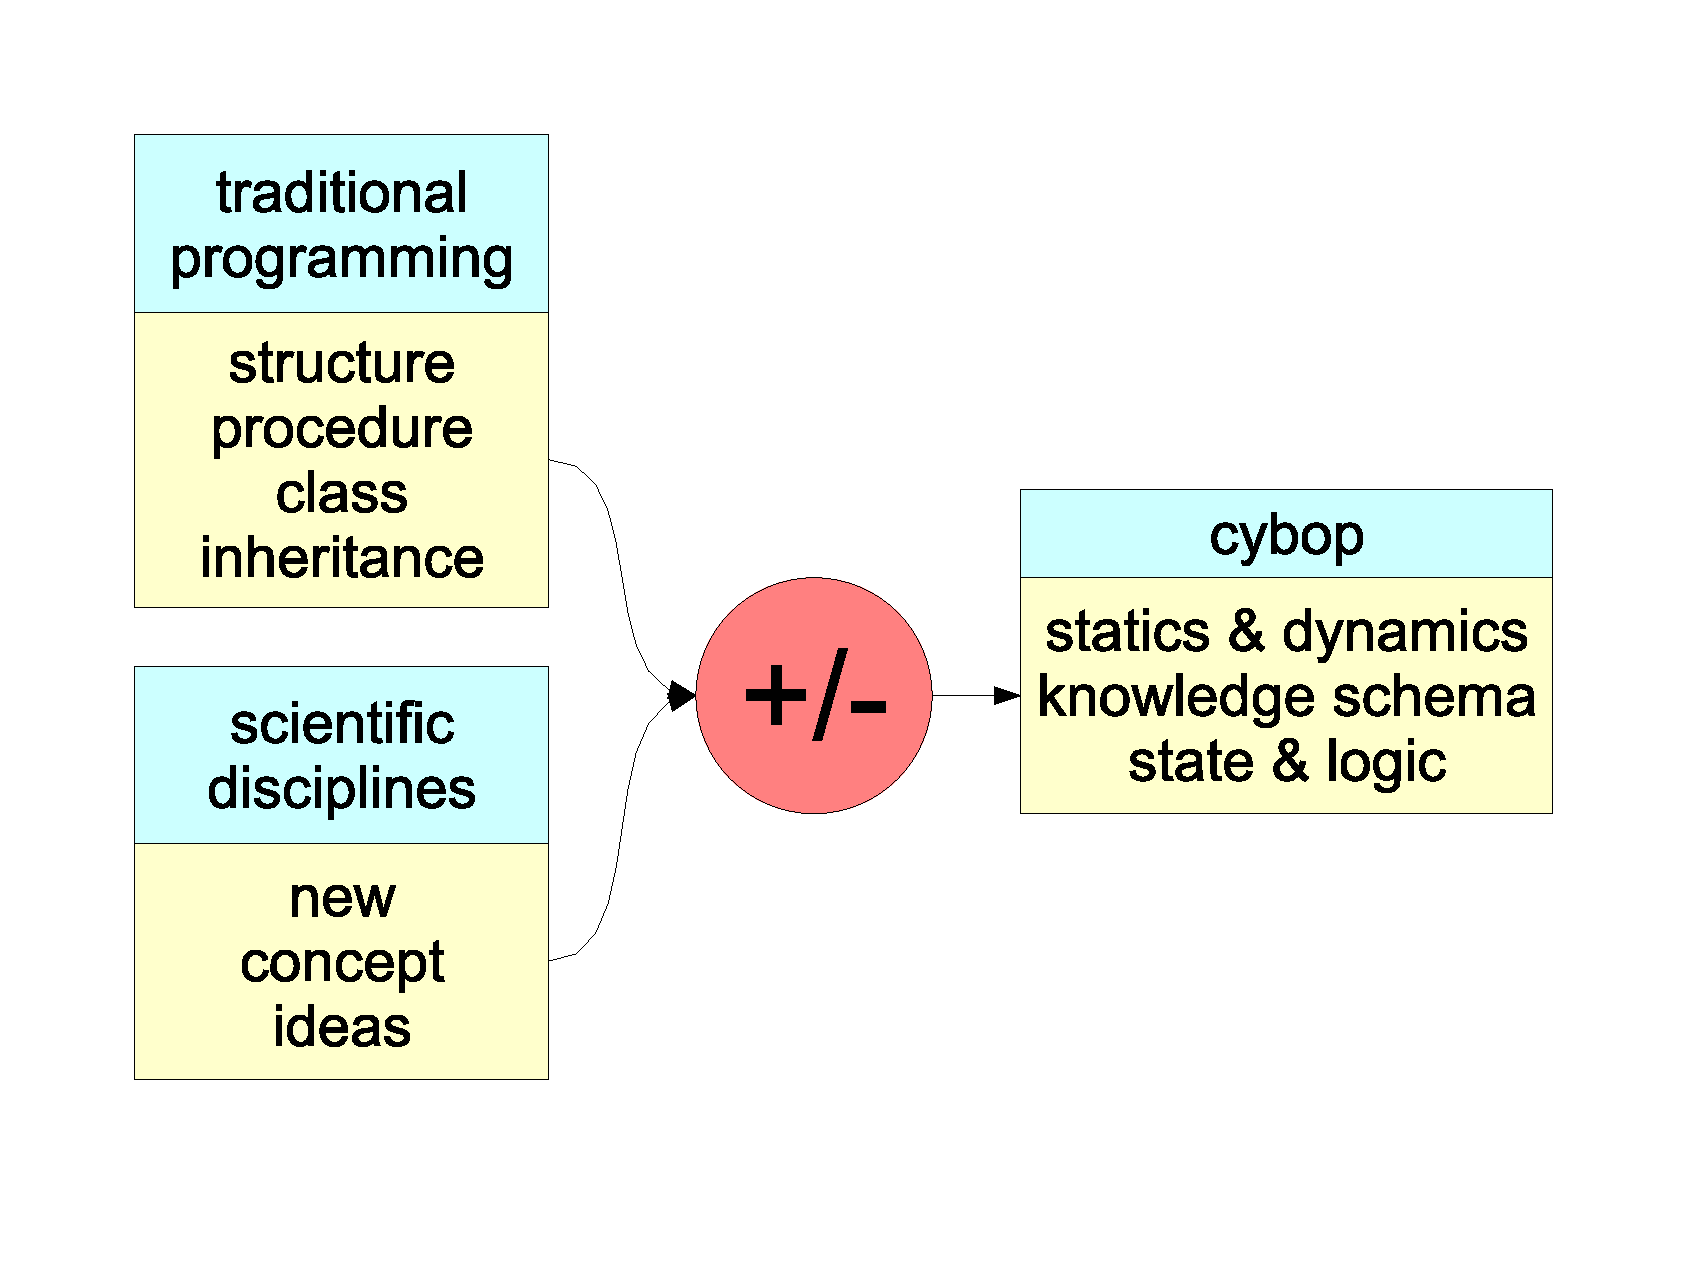
\includegraphics[scale=0.2]{vector/method.eps}
        \caption{Merger of Concepts}
        \label{method_figure}
    \end{center}
\end{figure}

However, these refactorings were only some of at least two dozens, since also
COP and the application of concerns, as well as other concepts applied later
(e.g. ontological structure implemented using the means of OOP) turned out to
have their deficiencies. According to the idea mentioned before, traditional
concepts were thus complemented, merged or revised with new concepts stemming
from other scientific disciplines (figure \ref{method_figure}), whenever a
classical design solution became unsatisfying.

Over the creation of a framework called \emph{ResMedLib}, which encapsulated
general application functionality, the prototype development finally ended up
in a complete reengineering: most of the functionality formerly residing in the
framework was moved into an interpreter (section \ref{cyboi_heading}) written
in the \emph{C} programming language; the actual application knowledge, on the
other hand, was put into special files, for which an
\emph{Extensible Markup Language} (XML)-based language (section
\ref{cybol_heading}) was defined.

Since problems did not occur in a predictable way, while developing the
mentioned prototype application, their presentation in order of appearance
would be rather confusing. An adapted structure of sections is therefore used
in this article, which first describes a number of observed discrepancies
(section \ref{existing_problems_heading}), then reflects on the most essential
new concepts (section \ref{reflexions_on_concepts_heading}), before it later
explains how these were implemented in practice (section
\ref{practical_proof_heading}).

